IRSTI 28.23.15

{\bfseries TRAFFIC SIGN RECOGNITION IN CHALLENGING WEATHER CONDITIONS USING
CONVOLUTIONAL NEURAL NETWORKS}

{\bfseries \textsuperscript{1}Zh.A. Batyr, \textsuperscript{1}B.S. Omarov,
\textsuperscript{1}G.Z. Ziyatbekova, \textsuperscript{2}A.D.
Mailybayeva}

\textsuperscript{1}Al-Farabi Kazakh National University, Almaty,
Kazakhstan,

\textsuperscript{2}Khalel Dosmukhamedov Atyrau University, Atyrau,
Kazakhstan,

е-mail: ziyatbekova1@gmail.com

The ability of autonomous driving systems to recognize traffic signs in
a variety of environmental conditions is crucial to their reliability.
This study uses convolutional neural networks (CNNs) to provide a novel
method for improving the accuracy of traffic sign recognition systems
under challenging weather situations. The research focuses on developing
a CNN-based model that is trained using the augmented German Traffic
Sign Recognition Benchmark (GTSRB) dataset, which contains over 50,000
labeled images of road signs across 43 categories. To attempt to
overcome the limitations of traditional CNN models under adverse
environmental conditions, this work presents adaptive feature extraction
layers that are especially made to reduce visibility problems brought on
by rain, fog, and snow. By taking a comprehensive approach, the model
uses advanced data augmentation methods to simulate different weather
scenarios, greatly increasing the diversity of the training dataset.
Through an analysis of theoretical and practical aspects, the study
demonstrates how CNNs enhance the accuracy and efficiency of road sign
detection systems in a different weather condition. Research evaluates
the model\textquotesingle s effectiveness using metrics such as
precision, recall, and F1-score, proving its capability to reduce false
positives and accurately detect relevant road sign instances.
Additionally, the paper highlights the importance of careful dataset
preparation and augmentation, model optimization, and training
enhancements to improve the performance of road sign detection systems.
The results of this research offer benefits for intelligent transport
systems, autonomous driving, and road safety, pointing towards further
advancements in precise and dependable road sign recognition technology.

Keywords: CNN, traffic sign detection, artificial intelligence, image
analysis, classification

{\bfseries РАСПОЗНАВАНИЕ ДОРОЖНЫХ ЗНАКОВ В СЛОЖНЫХ ПОГОДНЫХ УСЛОВИЯХ С
ИСПОЛЬЗОВАНИЕМ СВЕРТОЧНЫХ НЕЙРОННЫХ СЕТЕЙ}

{\bfseries \textsuperscript{1}Ж.А. Батыр, \textsuperscript{1}Б.С. Омаров,
\textsuperscript{1}Г.З. Зиятбекова, \textsuperscript{2}А.Д. Майлыбаева}

\textsuperscript{1}Казахский национальный университет имени аль-Фараби,
Алматы, Казахстан,

\textsuperscript{2}Атырауский университет имени Х. Досмухамедова,
Атырау, Казахстан,

е-mail: ziyatbekova1@gmail.com

В исследовании рассматривается использование сверточных нейронных сетей
(CNN) для улучшения систем распознавания дорожных знаков, особенно в
сложных погодных условиях. В исследовании, основанном на новой модели
CNN, используется расширенный набор данных немецкого теста распознавания
дорожных знаков (GTSRB), который содержит более 50 000 изображений с
надписями, охватывающих 43 категории. В модели представлены адаптивные
слои выделения объектов, предназначенные для устранения проблем с
видимостью, вызванных такими погодными факторами, как дождь, туман и
снег. Для моделирования различных погодных сценариев применяются
передовые методы увеличения объема данных, что увеличивает разнообразие
обучающего набора данных. Это исследование не только рассматривает
теоретические и практические усовершенствования, предоставленные CNNs
для обнаружения дорожных знаков в неблагоприятных условиях, но и
проверяет эффективность модели с помощью таких показателей, как
точность, отзывчивость и показатель F1. Результаты подтверждают
эффективность модели в минимизации ложных срабатываний и точной
идентификации дорожных знаков. В документе подчеркивается важность
тщательной подготовки набора данных, оптимизации моделей и
усовершенствования обучения для повышения производительности системы
обнаружения. Это положительно сказывается на интеллектуальных
транспортных системах, автономном вождении и безопасности дорожного
движения, что свидетельствует о будущем прогрессе в области надежных
технологий распознавания дорожных знаков.

{\bfseries Ключевые слова:} CNN, распознавание дорожных знаков,
искусственный интеллект, анализ изображений, классификация.

{\bfseries КОНВОЛЮЦИЯЛЫҚ НЕЙРОНДЫҚ ЖЕЛІЛЕРДІ КӨМЕГІМЕН ҚИЫН АУА-РАЙЫ
ЖАҒДАЙЛАРЫНДА ЖОЛ БЕЛГІЛЕРІН ТАНУ}

{\bfseries \textsuperscript{1}Ж.А. Батыр, \textsuperscript{1}Б.С. Омаров,
\textsuperscript{2}Г.З. Зиятбекова, \textsuperscript{2}А.Д. Майлыбаева}

\textsuperscript{1}әл-Фараби атындағы Қазақ ұлттық университеті, Алматы,
Қазақстан,

\textsuperscript{2}Халел Досмұхамедов атындағы Атырау университеті,
Атырау, Қазақстан,

е-mail: ziyatbekova1@gmail.com

Зерттеу жол белгілерін тану жүйелерін жақсарту үшін, әсіресе қиын
ауа-райында, конволюциялық нейрондық желілерді (CNN) пайдалануды
зерттейді. CNN-ге негізделген жаңа модельді пайдалана отырып, зерттеу 43
санатты қамтитын 50 000-нан астам таңбаланған кескіндерді қамтитын неміс
жол белгілерін тану стандартының (GTSRB) кеңейтілген деректер жинағын
пайдаланады. Модель жаңбыр, тұман және қар сияқты ауа райы
элементтерінен туындаған көріну мәселелерін азайтуға арналған адаптивті
мүмкіндіктерді шығару қабаттарын ұсынады. Деректерді көбейтудің
жетілдірілген әдістері ауа-райының әртүрлі сценарийлерін модельдеу үшін
қолданылады, бұл оқу деректер жиынтығының әртүрлілігін байытады. Бұл
зерттеу қолайсыз жағдайларда жол белгілерін анықтау үшін CNN-ге ұсынған
теориялық және практикалық жақсартуларды зерттеп қана қоймайды, сонымен
қатар модельдің өнімділігін дәлдік, еске түсіру және F1-ұпайы сияқты
көрсеткіштер арқылы тексереді. Нәтижелер модельдің жалған позитивтерді
азайтудағы және жол белгілерін дәл анықтаудағы тиімділігін растайды.
Мақалада деректер жиынтығын мұқият дайындаудың, модельдерді
оңтайландырудың және анықтау жүйесінің өнімділігін арттыру үшін оқытуды
жетілдірудің маңыздылығы атап өтілген. Бұл интеллектуалды көлік
жүйелеріне, автономды жүргізуге және жол қауіпсіздігіне оң ықпал етеді,
бұл жол белгілерін танудың сенімді технологиясының болашақтағы
ілгерілеуін көрсетеді.

{\bfseries Түйін сөздер:} CNN, жол белгілерін анықтау, жасанды интеллект,
кескінді талдау, жіктеу.

{\bfseries Introduction.} Traffic sign recognition is a critical component
in the development of intelligent transportation systems and autonomous
vehicles. Accurate detection and interpretation of road signs enable
automated systems to make informed decisions, thereby enhancing road
safety and efficiency {[}1{]}. However, the challenges in traffic sign
recognition primarily arise from variable lighting conditions,
occlusions, and environmental factors such as weather conditions that
can significantly degrade the visibility of traffic signs {[}2{]}.

The primary objective of this study is to enhance the accuracy of
traffic sign recognition systems under challenging weather conditions
using Convolutional Neural Networks (CNNs). This involves developing and
testing a CNN-based model that can effectively handle adverse weather
conditions such as rain, fog, and snow. The study aims to introduce
adaptive feature extraction layers and advanced data augmentation
methods to simulate different weather scenarios, thus increasing the
robustness and reliability of traffic sign detection systems in
real-world environments.

{\bfseries Literary Review.} Convolutional Neural Networks (CNNs) have
become the standard in the field of image recognition and are
increasingly being applied to traffic sign recognition due to their
ability to extract high-level features from visual inputs {[}3{]}. The
German Traffic Sign Recognition Benchmark (GTSRB) dataset, with its
comprehensive set of over 50,000 images spanning 43 classes, provides a
solid basis for training and evaluating traffic sign recognition systems
{[}4{]}.

Many models of traffic recognition systems have been proposed over the
past decade {[}5-7{]}. Generally, these systems operate through
detection and recognition stages. While CNNs perform exceptionally well
under standard conditions, their efficiency decreases in adverse weather
conditions such as rain, fog, and snow, which obscure and alter the
appearance of signs {[}8{]}. Addressing these challenges requires the
development of effective models that can adapt to and correct for
environmental distortions.

This research builds upon existing methodologies by enhancing CNN
architectures to improve recognition accuracy in challenging weather
conditions. By integrating adaptive feature extraction layers that
respond to weather-specific disturbances, this study aims to
significantly contribute to the reliability of autonomous driving
technologies under diverse operating conditions {[}9{]}. Furthermore, it
underscores the importance of meticulous model training and dataset
curation, as these are crucial for optimizing performance and ensuring
the system\textquotesingle s real-world applicability {[}10{]}.

{\bfseries Methods and Materials.} The GTSRB dataset that was used for this
study, contains 51893 images categorized into 43 classes of traffic
signs showing in Fig. 1. The size of the images in dataset varies
between 15x15 and 222x193 pixels. All these images were taken in real
environment, including bad weather conditions and different light
illumination. Some images are low resolution and can be difficult to
recognize.

\begin{figure}[H]
	\centering
	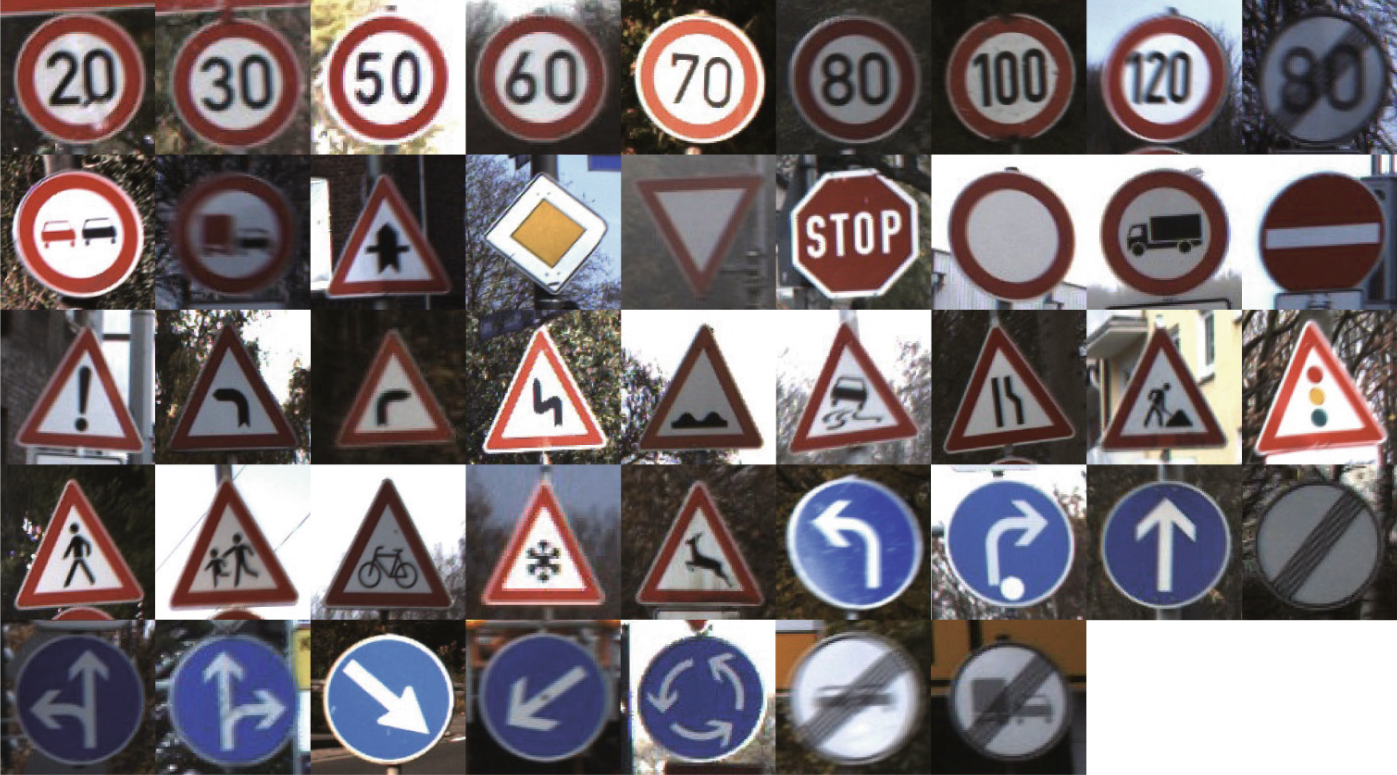
\includegraphics[width=0.8\textwidth]{assets/57}
	\caption*{}
\end{figure}

{\bfseries Figure 1- The 43 traffic sign classes in the dataset}

Existing datasets are limited in terms of their size and challenging
condition coverage, which motivated us to augment images using image
augmentation methods. To simulate adverse weather conditions, additional
image preprocessing techniques such as artificial rain, fog, and snow
overlays were applied to the original dataset. This augmentation aimed
to provide a diversified set of training images reflecting real-world
challenges. There are various types of image augmentations done to
increase the image corpus for training neural networks {[}11{]}.

Using OpenCV library we created image augmentation methods for
processing images and applying weather condition filters to them. These
augmentations simulate real-world environmental effects that can impede
traffic sign recognition, such as rain, fog, snow, shadows, and lighting
variations. The purpose of these augmentations is to create a diverse
training set that allows the model to learn and adapt to different
visual disturbances that are common in adverse weather conditions.

To create rain augmentation, we used OpenCV's line function to generate
small lines all over the image. By adding random slants in the rain
drops and reducing image's brightness we can mimic rain or even heavy
rainfall. This method helps the model learn to recognize signs with
potential streaks and blurs caused by rain on the camera lens. Snow
effects were added by whitening dark parts of the image by changing
pixel values of lightness channel in image's color space. Fog was
simulated by adding a uniform or gradient-based haze over the images,
using varying intensities of white overlay. The opacity level was
adjusted to create different densities of fog, from light mist to dense
fog, which can obscure the visibility of traffic signs. In addition to
specific weather condition augmentations, we implemented a random
augmentation pipeline where each image could undergo a combination of
the above effects. Fig. 2 shows examples of using these augmentation
methods. By using these augmentation techniques, our training dataset
was enriched with a variety of challenging conditions, preparing the CNN
model to perform reliably in diverse and unpredictable real-world
environments.

\begin{figure}[H]
	\centering
	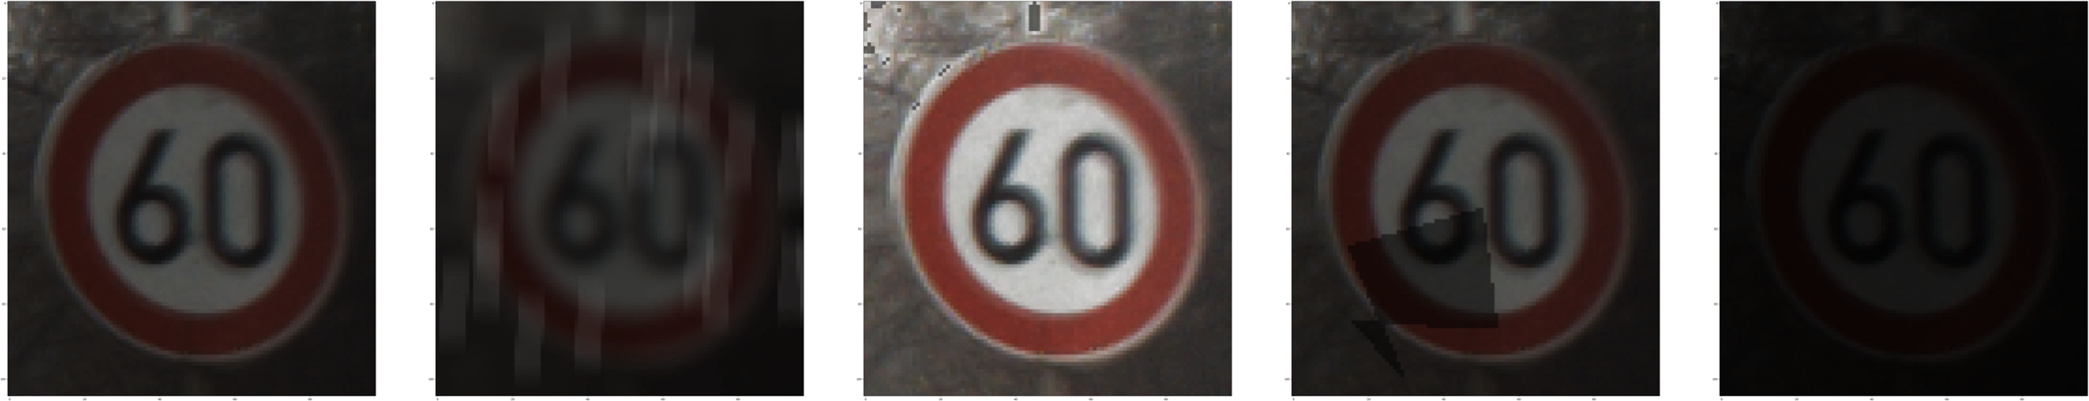
\includegraphics[width=0.8\textwidth]{assets/58}
	\caption*{}
\end{figure}

{\bfseries Figure 2 - Applying augmentations to traffic sign image}

These augmentation methods not only diversified the training dataset but
also significantly contributed to the model\textquotesingle s ability to
generalize from the training data to real-world scenarios, ensuring
reliable performance across a spectrum of adverse conditions. This
approach underscores the importance of comprehensive and realistic data
augmentation in developing advanced computer vision systems for
autonomous driving and related applications. The dataset was classified
using the classification function included in the python scikit-learn
library. 80\% of the data was used for training and 20\% for testing.

Fig. 3 illustrates the architectural design of the proposed
Convolutional Neural Network (CNN) for traffic sign recognition,
showcasing a network structure comprised of 12 layers.

\begin{figure}[H]
	\centering
	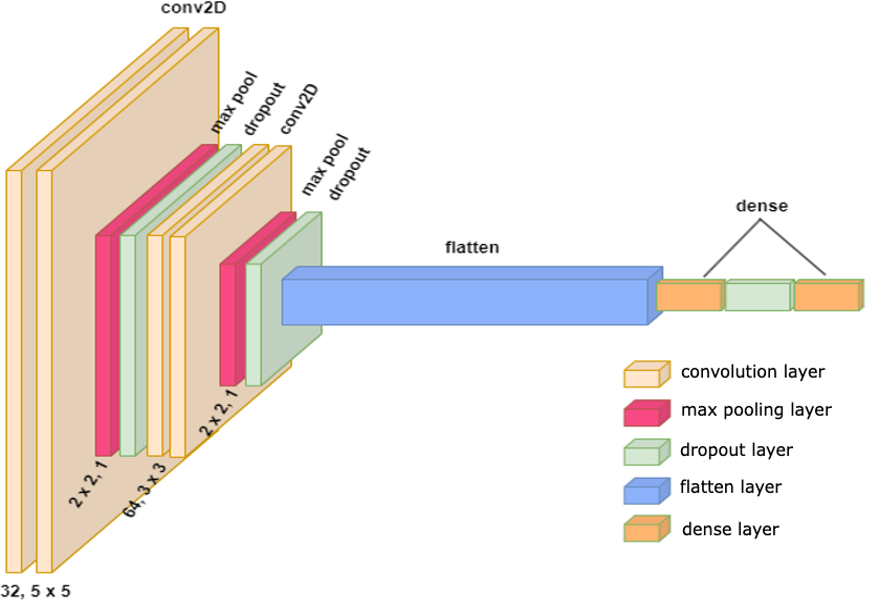
\includegraphics[width=0.8\textwidth]{assets/59}
	\caption*{}
\end{figure}

{\bfseries Figure 3- Applying augmentations to traffic sign image}

The initial input to this model consists of color images sized at 30x30
pixels. CNN model contains 4 convolutional layers, max pooling, dropout
and flatten layers. The output of last fully connected layer is fed to a
43-way softmax which produces a distribution over the 43 class traffic
sign labels. In CNN architectures, combining layers can be used to
reduce the size of the input image, thereby accelerating computational
speed. This process involves adjusting two critical parameters: the
filter size denoted as \textquotesingle f\textquotesingle{} and the
stride represented as \textquotesingle s.\textquotesingle{} The
amalgamation of layers results in reduced sensitivity to pixel
positions, often employing common values such as f=2 and s=2 {[}12{]}.
However, it is essential to note that this size reduction also
corresponds to a decrease in the number of coefficients under scrutiny,
affecting computational resources accordingly. Within the CNN
architecture, the convolutional filter kernels are trained using
observed data, learning from a set of established examples. At each
hierarchical level, CNN undertakes sampling operations to aggregate
feature responses from neighboring pixels. These operations enable CNN
to master spatially invariant functions, ones that do not rely on object
placement within the images {[}13{]}.

In the field of machine learning and classification tasks, evaluation
metrics are essential for measuring the performance and efficacy of a
model. Metrics such as accuracy, precision, recall, and the F-score are
fundamental in determining a model\textquotesingle s predictive power
and its capacity to generalize across new data. These parameters play a
crucial role in quantifying how effectively a model can handle and
predict on data it has not previously encountered {[}14{]}.

{\bfseries Results.} We trained our network using the TensorFlow machine
learning framework, utilizing the Adam optimizer with a learning rate of
0.001. The batch size was set to 32, and to mitigate overfitting,
dropout regularization was applied to the first two fully connected
layers. The proposed CNN model underwent testing over 15 epochs. To
evaluate the effectiveness of the neural network post-training, our
model features a 12-layer convolutional neural network designed for the
detection and recognition of traffic signs. The initial layer receives
an image in a 30x30 pixel resolution in RGB color format. Subsequently,
the second layer employs a Conv2D operation with the ReLU activation
function. The third layer utilizes a max pooling operation (MaxPool2D),
which takes various parameters including stride, kernel size, padding,
and return indices. Following this, the fourth layer also employs a
Conv2D with ReLU activation. The fifth layer once again applies
MaxPool2D. The sixth layer includes a flattening step to linearize the
inputs, followed by a densely connected layer, or dense layer, where
each neuron is fully connected to all neurons in the previous layer.
Finally, to enhance the accuracy and approach the ideal output, the
softmax function is used in the output dense layer, yielding the
probability of each class, where the recognized traffic sign is
determined. Fig. 4 shows accuracy and loss of the model.

\begin{figure}[H]
	\centering
	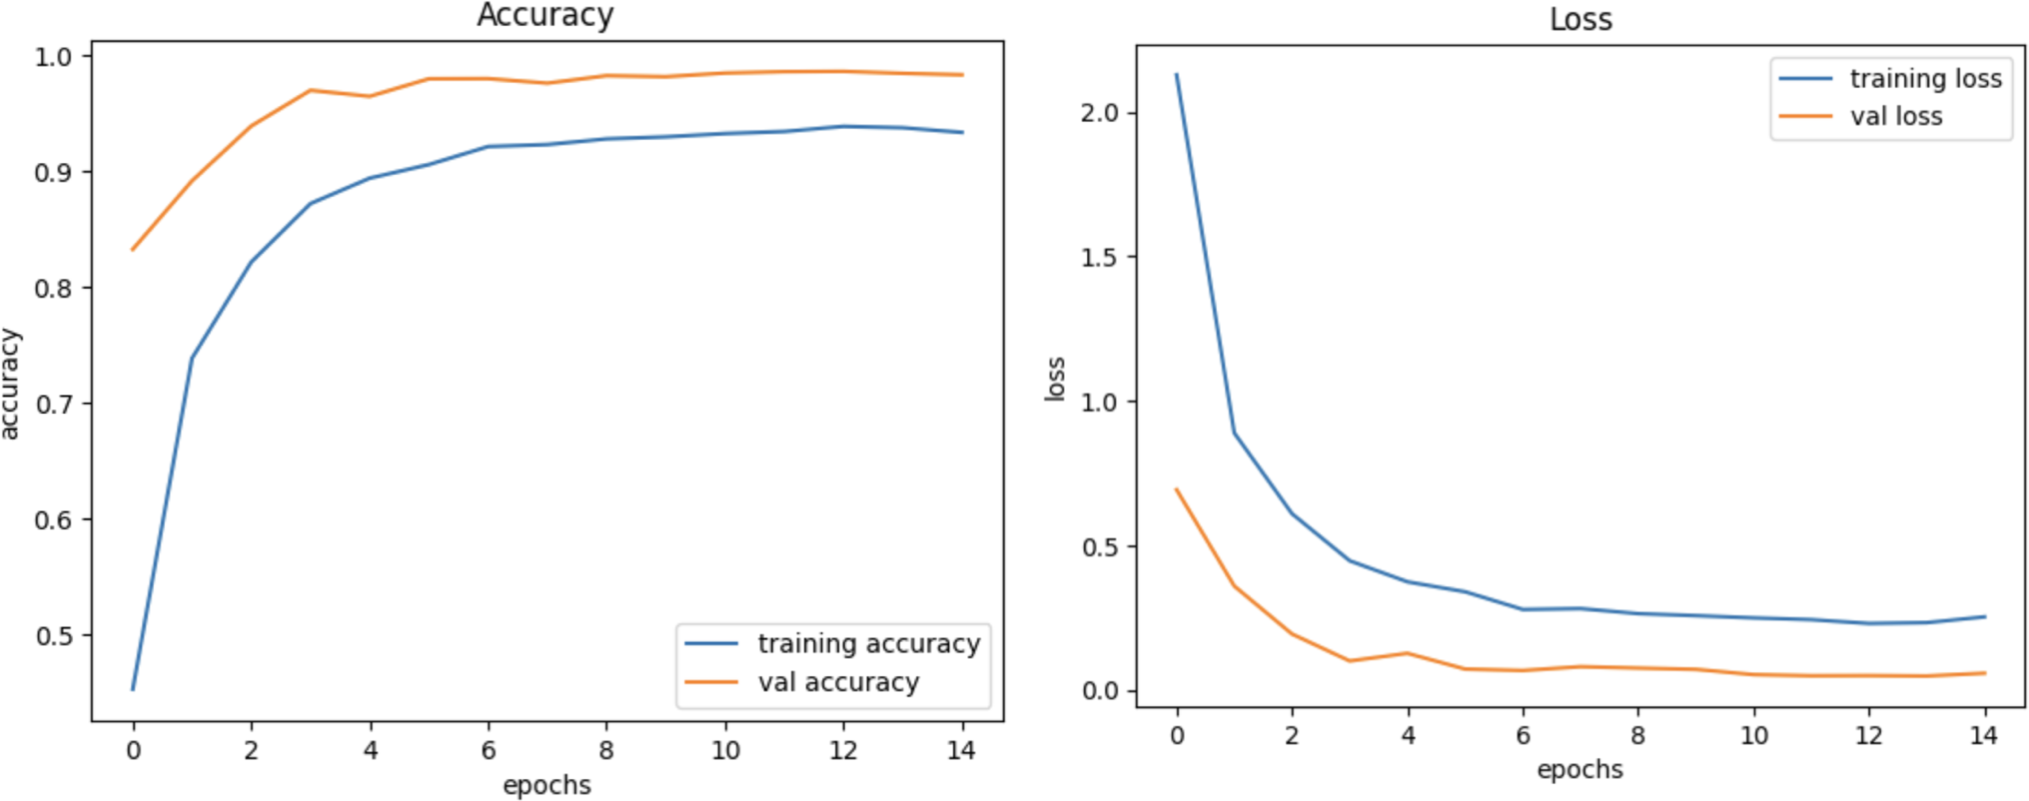
\includegraphics[width=0.8\textwidth]{assets/60}
	\caption*{}
\end{figure}

{\bfseries Figure 4 - Model accuracy and loss after training}

Table 1 shows the some of the quality indicators that are used to
evaluate test data in the model training stage. As an overall
performance measure, the global accuracy metric showed a great
achievement with an average of 95\% in the context of the test data.

\begin{quote}
{\bfseries Table 1 - Evaluation metrics after training stage}
\end{quote}

\begin{longtable}[]{@{}
  >{\raggedright\arraybackslash}p{(\columnwidth - 8\tabcolsep) * \real{0.2495}}
  >{\raggedright\arraybackslash}p{(\columnwidth - 8\tabcolsep) * \real{0.2046}}
  >{\raggedright\arraybackslash}p{(\columnwidth - 8\tabcolsep) * \real{0.1820}}
  >{\raggedright\arraybackslash}p{(\columnwidth - 8\tabcolsep) * \real{0.1820}}
  >{\raggedright\arraybackslash}p{(\columnwidth - 8\tabcolsep) * \real{0.1820}}@{}}
\toprule\noalign{}
\endhead
\bottomrule\noalign{}
\endlastfoot
& {\bfseries Precision} & {\bfseries Recall} & {\bfseries F1-score} &
{\bfseries Support} \\
{\bfseries Class 1} & 0,98 & 0,95 & 0,97 & 60 \\
{\bfseries Class 2} & 0,85 & 0,97 & 0,91 & 720 \\
{\bfseries Class 3} & 0,98 & 0,89 & 0,94 & 750 \\
{\bfseries Class 4} & 0,88 & 0,85 & 0,87 & 450 \\
{\bfseries Class 5} & 0,99 & 0,89 & 0,94 & 660 \\
\end{longtable}

Additionally, a more thorough evaluation metric for the first class in
the task of classifying traffic signs produced the following significant
outcomes:

The F1-score, a composite measure that achieves a balance between recall
and precision, reached a remarkable 97\%. This accomplishment
demonstrates the model\textquotesingle s strong performance in reducing
false positives and correctly identifying pertinent cases.

These clarified results add to the body of knowledge regarding machine
learning and classification efforts by highlighting the effectiveness
and dependability of the model\textquotesingle s performance in the task
of classifying road signs.

The suggested CNN model\textquotesingle s accuracy and strength hold
practical implications for the development of intelligent transportation
infrastructure and autonomous driving systems. Autonomous vehicles must
be able to recognize traffic signs accurately in inclement weather to
make safe and sensible decisions in real-world situations. This
dependability is essential for lowering accident rates and improving
general traffic safety, especially in inclement weather conditions when
human drivers may find it difficult to see.

Furthermore, the approach that makes use of thorough data augmentation
techniques and adaptive feature extraction layers offers a foundation
that may be used for other elements of autonomous driving, like lane
recognition and pedestrian detection. This flexibility improves
CNNs\textquotesingle{} overall usefulness in a range of intelligent
transportation system applications. These results are practically
significant because they have the potential to enhance the reliability
and performance of autonomous cars, which will ultimately lower the
number of traffic accidents and increase the effectiveness of
transportation networks.

{\bfseries Discussion.} The results of the experimental stage provide
compelling evidence of the effectiveness of the convolutional neural
network (CNN) architecture in recognizing traffic signs under various
challenging weather conditions. The application of adaptive feature
extraction layers, customized augmentation methods, and calculated
dropout regularization significantly improved the resilience and
accuracy of the model.

The adaptive feature extraction layers played a crucial role in
mitigating the visual distortions caused by adverse weather conditions.
Adaptive methods in CNNs enable flexible modifications to filters that
respond to specific environmental variables, as discussed in previous
works {[}15{]}. The study\textquotesingle s ability to reduce the impact
of snow, fog, and rain on sign visibility demonstrates the advantage of
such adaptive approaches in real-world situations {[}16{]}.

Comparisons with baseline models described in contemporary research
showed an improvement in handling variably degraded images due to
weather conditions. These comparisons validate the
model\textquotesingle s design and highlight its potential to surpass
existing systems in both accuracy and reliability under adverse
conditions {[}17{]}.

The effectiveness of the CNN model is underscored by achieving a 95\%
accuracy rate in recognizing traffic signs, a notable improvement over
general CNN models used in similar contexts. This high level of
performance was measured using standard evaluation metrics such as
precision, recall, and the F1-score, which are critical for assessing
the predictive capabilities and generalization power of the model
{[}18{]}. Precision measures the accuracy of the positive predictions
made by the model, while recall reflects the model\textquotesingle s
ability to detect all relevant instances. The F1-score provides a
balance between precision and recall, offering a holistic view of the
model's efficiency {[}19-20{]}.

In summary, the study demonstrates that planned architectural
improvements combined with precise training dataset curation can
significantly enhance CNN performance in real-world applications like
traffic sign recognition. The methodologies used under artificially
challenging conditions suggest promising prospects for use in
self-driving systems, where dependability and security hold vital
importance.

{\bfseries Conclusions.} This study has effectively shown that a modified
convolutional neural network (CNN) architecture can accurately and
efficiently interpret traffic signs in inclement weather. Using
substantial data augmentation techniques and adaptive feature extraction
layers, we have improved the model\textquotesingle s resistance to
environmental influences that usually cause visual recognition systems
to malfunction. By using dropout regularization, the model has been able
to prevent overfitting and maintain good generalization to new, untested
data.

Our results show that planned architectural improvements combined with
precise training dataset curation can significantly improve CNN
performance on real-world applications like traffic sign recognition.
The effective usage of these methodologies under artificially
challenging conditions implies promising prospects for use in
self-driving systems, were dependability and security hold vital
importance.

In conclusion, our research advances the field of autonomous vehicles by
offering a more stable and reliable approach to traffic sign recognition
that can work well in despite of environmental challenges. This
development represents a step toward the eventualization of completely
autonomous cars that can navigate safely under any circumstance,
improving transportation efficiency and road safety.

{\bfseries References}

1.Escalera A. de la, Armingol J.M., Mata M. Traffic sign recognition and
analysis for intelligent vehicles // Image and vision computing.
-2003.-Vol. 21(3). - Р. 247-258. DOI 10.1016/S0262-8856(02)00156-7

2.Ahmed S., Kamal U., Hasan M. K. DFR-TSD: A deep learning based
framework for robust traffic sign detection under challenging weather
conditions // IEEE Transactions on Intelligent Transportation Systems. -
2022. -Vol.23 (6). -Р. 5150-5162. DOI: 10.1109/TITS.2020.3048878

3.Shustanov, A., Yakimov, P. CNN design for real-time traffic sign
recognition // Procedia engineering. -2017. -Vol. 201. -Р. 718-725. DOI
10.1016/j.proeng.2017.09.594

4.Haloi, M. Traffic sign classification using deep inception based
convolutional networks. -2016. DOI 10.48550/arXiv.1511.02992

5.Nguwi, Y.Y., Kouzani, A.Z. Detection and classification of road signs
in natural environments // Neural Comput, 2008. - Vol. 17. - Р.
265--289. DOI:10.1007/s00521-007-0120-z

6.Sermanet, P., \& LeCun, Y. Traffic sign recognition with multi-scale
convolutional networks. In The 2011 international joint conference on
neural networks//IEEE.-2011.-Р.2809-2813.

DOI 10.1109/IJCNN.2011.6033589

7.Tang, S., \& Huang, L. L. Traffic sign recognition using complementary
features // In 2013 2nd IAPR Asian conference on pattern recognition. -
2013. -Р. 210-214. DOI 10.1109/ACPR.2013.63

8.Dang T. P., Tran N. T., To, V. H., \& Tran Thi, M. K. Improved YOLOv5
for real-time traffic signs recognition in bad weather conditions // The
Journal of supercomputing. -2023. -Vol. 79. -Iss. 10. -Р. 10706-10724.
DOI 10.1007/s11227-023-05097-3

9.Puli, M. S., Sunitha, M., Aluri, O. S. B., Jain, D. R., Rayabharapu,
M., \& Venkatesh, M. Deep Learning-Based Framework For Robust Traffic
Sign Detection Under Challenging Weather Conditions // Journal of Survey
in Fisheries Sciences. -2023. -Vol. 23 (6) -Р. 5150-5162.

DOI 10.1109/TITS.2020.3048878

10.Qian, R., Yue, Y., Coenen, F., \& Zhang, B. Traffic sign recognition
with convolutional neural network based on max pooling positions // In
2016 12th International conference on natural computation, fuzzy systems
and knowledge discovery (ICNC-FSKD).-2016.-Р.578-582. DOI
10.1109/FSKD.2016.7603237

11.Bloice, M. D., Stocker, C., \& Holzinger, A. Augmentor: an image
augmentation library for machine learning // Computer Vision and Pattern
Recognition.-2017.-DOI 10.48550/arXiv.1708.04680

12.Murphy, J. An overview of convolutional neural network architectures
for deep learning. Microway. - Inc, 2016.- Р.1-22. URL:
https://www.semanticscholar.org/paper/An-Overview-of-Convolutional-Neural-Network-for-Murphy/64db333bb1b830f937b47d786921af4a6c2b3233

13.Traore, B. B., Kamsu-Foguem, B., \& Tangara, F. (2018). Deep
convolution neural network for image recognition // Ecological
informatics. - 2018. -Vol. 48.- Р. 257-268. DOI
10.1016/j.ecoinf.2018.10.002

14.Yacouby, R., \& Axman, D. Probabilistic extension of precision,
recall, and f1 score for more thorough evaluation of classification
models // In Proceedings of the first workshop on evaluation and
comparison of NLP systems. - 2020. -Р. 79-91. DOI
10.18653/v1/2020.eval4nlp-1.9

15.Yao, Z., Song, X., Zhao, L., \& Yin, Y. (2021). Real-time method for
traffic sign detection and recognition based on YOLOv3-tiny with
multiscale feature extraction // Proceedings of the Institution of
Mechanical Engineers, Part D: Journal of Automobile Engineering. -2021.-
Vol. 235(7)- Р. 1978-1991.

DOI 10.1177/0954407020980559

16.Yucong, S., \& Shuqing, G. (2021). Traffic sign recognition based on
HOG feature extraction // Journal of Measurements in Engineering. -
2021.- Vol. 9 (3)-Р. 142-155. DOI 10.21595/jme.2021.22022

17.Feng, L., \& Jia, Y. Traffic sign recognition based on YOLOX in
extreme weather // In 2022 Global Conference on Robotics, Artificial
Intelligence and Information Technology (GCRAIT). -2022. - Р. 299-303.
DOI: 10.1109/GCRAIT55928.2022.00070

18.Luo, H., Yang, Y., Tong, B., Wu, F., \& Fan, B. Traffic sign
recognition using a multi-task convolutional neural network // IEEE
Transactions on Intelligent Transportation Systems. -2017. - Vol. 19. -
Iss. 4. -- Р. 1100-1111. DOI 10.1109/TITS.2017.2714691

19.Lin Z., Yih M., Ota J.M., Owens J., Muyan-Ozcelik, P. Benchmarking
Deep Learning Frameworks and Investigating FPGA Deployment for Traffic
Sign Classification and Detection // IEEE Transactions on Intelligent
Vehicles. - 2019. - Vol. 4(3) - Р. 385-395. DOI 10.1109/TIV.2019.2919458

20.Sun, P., Zhang, R.Y., Jiang, T., Kong, C., Xu, W., Zhan, M.,
Tomizuka, L., Li, Z., Yuan, C., Wang \& Luo, P. Sparse R-CNN: End-to-end
object detection with learnable proposals // Proceedings of the IEEE/CVF
conference on computer vision and pattern recognition. -2021.-
https://doi.org/10.48550/arXiv.2011.12450

\emph{{\bfseries Information about the authors}}

Zh.Batyr - graduate student at Al-Farabi Kazakh National University,
e-mail: zhan.batyr01@gmail.com;

B.Omarov - PhD, Associate Professor Al-Farabi Kazakh National
University; e-mail: batyahan@gmail.com;

G.Ziyatbekova -PhD, Acting Associate Professor Al-Farabi Kazakh National
University, Corresponding author; e-mail: ziyatbekova1@gmail.com;

A/Mailybayeva -Candidate of Physical and Mathematical Sciences,
Associate Professor of the Department of Informatics, Khalel
Dosmukhamedov Atyrau University, e-mail: mjkka@mail.ru

\emph{{\bfseries Сведения об авторах}}

Батыр Ж.А.докторант Казахского национального университета имени
аль-Фараби, e-mail: zhan.batyr01@gmail.com;

Омаров Б.С.- PhD, доцент, Казахский национальный университет имени
аль-Фараби, e-mail: batyahan@gmail.com;

Зиятбекова Г.З.PhD - и.о. доцента Казахского национального университета
имени аль-Фараби, e-mail: ziyatbekova1@gmail.com;

Майлыбаева А.Д.-кандидат физико-математических наук, ассоциированный
профессор кафедры Информатики, Атырауский университет имени Халела
Досмухамедова, e-mail: mjkka@mail.ru
